\documentclass[tikz]{standalone}
\usepackage{amsmath}
\usepackage{mathtools}
\usepackage{helvet}
\usepackage[T1]{sansmath}
\usetikzlibrary{arrows,decorations.markings}
\renewcommand{\familydefault}{\sfdefault}
\normalfont

\begin{document}
\begin{sansmath}

\tikzstyle{circ} = [circle,draw,thick,fill=blue!10,minimum size = 1cm,thick]
    
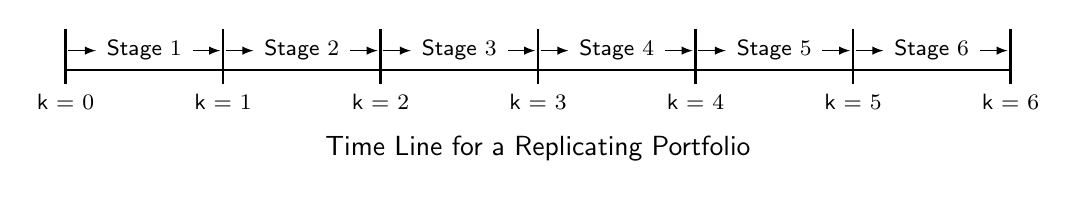
\begin{tikzpicture}[auto]
    %\draw[help lines] (0,2) grid (15,-2);
    
    \node (xlabel) at (6,-1) {Time Line for a Replicating Portfolio};
    
    \draw [thick] (0,0)--(6*2,0);
    \foreach \k in {0,...,6}
    	\draw [shift={(2*\k,0)},thick] (0pt,15pt)--(0pt,-5pt) node[below] {\footnotesize k = $\k$};
    \foreach \k in {1,...,6}{
    	\draw [thick] (2*\k-1,0) node[above] {\footnotesize Stage $\k$};
    	\draw [-latex] (2*\k-2,0.25) ++(1pt,0) --++(10pt,0);
    	\draw [latex-] (2*\k,0.25) ++(-1pt,0) --++ (-10pt,0);
    }
    	
\end{tikzpicture}

\end{sansmath}
\end{document}
